\documentclass{article}

\usepackage[ruled,vlined]{algorithm2e} % pseudo-code
\SetKw{KwTo}{à} % mots clés pseudo-code en français
\SetKwFor{Pour}{pour}{faire}{fin}
\SetKwIF{Si}{SinonSi}{Sinon}{si}{alors}{sinon si}{sinon}{fin si}
\SetKw{Retour}{retourner}
\SetKw{Donnees}{Données:}
\SetKw{Resultat}{Résultat:}
\usepackage{csquotes}
\usepackage{parskip}
\usepackage{graphicx} % Required for inserting images
\usepackage{wrapfig}
\usepackage{tikz} %tracer graphes
\usepackage{xcolor} %couleurs
\usepackage{mathrsfs} % symboles stylés
\usepackage{amsmath} %vecteurs (entre autres)
\usepackage{stmaryrd} % intervalle d'entiers
\usepackage{amssymb} % Nécessaire pour \mathbb, les symboles des ensembles
\usepackage{cancel} %barrer texte
\usepackage{amsthm,amsmath} %carré stylé à la fin démo
\usepackage{mdframed} % Pour les encadrements
\usepackage{hyperref} % hyperliens pour référencer les sections
\usepackage{pgfplots} % Package pour tracer des graphiques
\usepackage{float} % Pour placer les graphes
\pgfplotsset{compat=1.18} % Version compatible
\usepgfplotslibrary{polar} % coordonnées polaires
\usepackage[french]{babel} % pour les guillemets
\usepackage{mathtools}
\everymath{\displaystyle}
\usepackage[margin=3cm]{geometry}
\usepackage[T1]{fontenc}
\usepackage[backend=biber, language=french]{biblatex} % bibliographie en fr
\addbibresource{refs.bib}
\DeclareFontFamily{U}{wncy}{}
\DeclareFontShape{U}{wncy}{m}{n}{<->wncyr10}{}
\DeclareSymbolFont{mcy}{U}{wncy}{m}{n}
\DeclareMathSymbol{\Sha}{\mathord}{mcy}{"58} % symbole Sha du peigne de Dirac

\renewcommand{\proofname}{Démonstration} % Changer "Proof" en "Démonstration"

\setcounter{tocdepth}{2} % N'affiche que les section et subsection
\renewcommand{\contentsname}{Table des matières} % Titre personnalisé

% Style de l'encadré pour les définitions
\newmdenv[
    linewidth=1pt,
    roundcorner=5pt,
    linecolor=black,
    frametitle={Définition}
]{definitionbox}

% Style de l'encadré pour les théorèmes
\newmdenv[
    linewidth=1pt,
    roundcorner=5pt,
    linecolor=black,
    frametitle={Théorème}
]{theorembox}

% Style de l'encadré pour les propriétés
\newmdenv[
    linewidth=1pt,
    roundcorner=5pt,
    linecolor=black,
    frametitle={Propriété}
]{propertybox}

% Commande pour la remarque
\newcommand{\remarque}[1]{%
    \par\medskip
    \textbf{\textcolor{black}{Remarque.}} #1%
}

% Commande pour les corollaires
\newcommand{\corollaire}[1]{%
    \par\medskip
    \textbf{\textcolor{black}{Corollaire.}} #1%
    \par\medskip
}

% Commande pour la norme
\newcommand{\norm}[1]{\left\|#1\right\|}

% Commande pour le produit scalaire
\newcommand{\dotproduct}[2]{\langle #1, #2 \rangle}

\title{}
\author{}
%date




\begin{document}

\begin{titlepage}
    \centering
    \vspace*{4cm}
    
    {\Large \textsc{Sylvain Fraresso, Gaël Jean-Albert, \\Titouan Martineau, Thomas Saurel} \par}
    
    \vspace{2.5cm}

    \rule{0.6\textwidth}{0.4pt} \\ [0.5cm]
    {\Huge \bfseries Transformation de Fourier discrète \\ et applications à la compression \\ des sons et des images\par}
    \vspace{0.3cm}
    \rule{0.6\textwidth}{0.4pt}
    
    \vfill
    
    {\large \today \par}
    
\end{titlepage}

\newpage
\tableofcontents
\newpage

\section{Introduction}

\begin{wrapfigure}{r}{4.1cm}
\caption{Joseph Fourier (1768-1830).}\label{wrap-fig:1}
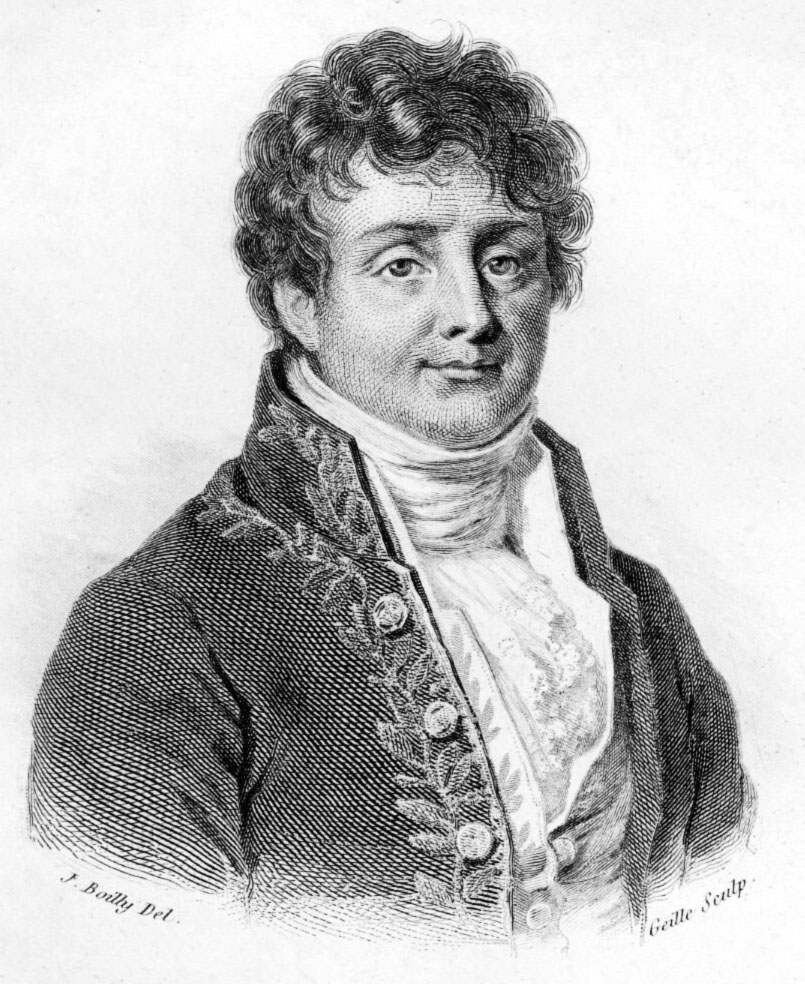
\includegraphics[width=4cm]{images/joseph_fourier.jpg}
\end{wrapfigure}

Au début du XIX\textsuperscript{ème}, le mathématicien Joseph Fourier travaille à la résolution de l'équation de la chaleur \cite{wiki-chaleur} , une équation aux dérivées partielles modélisant le phénomène de conduction thermique.
Dans le cadre de ses travaux, il introduit la notion de séries de Fourier, un développement en série trigonométrique des fonctions périodiques, et plus généralement la transformée de Fourier. Ces deux concepts seront alors étudiés minutieusement et donneront lieu à d'importantes découvertes en mathématiques, physique et informatique.

Le présent document aura pour objectif de formaliser la transformée de Fourier dans le cadre de la théorie du traitement du signal afin de comprendre comment cet outil peut être exploité en informatique pour la compression d'images numériques et de signaux sonores. On s'attardera en particulier sur l'implémentation et les applications de l'algorithme FFT (\og Fast Fourier Transform \fg pour transformée de Fourier rapide) permettant de calculer très efficacement des transformées de Fourier.

\section{Les signaux}

\subsection{Définition}

Commençons par introduire la notion de signal. On appelle \textbf{signal analogique} ou \textbf{continu}, une fonction de $\mathbb{R}$, représentant le temps, vers $\mathbb{C}$ \cite{wiki-signal} . Bien que les mesures physiques soient réelles, un signal complexe permet de conserver la \textbf{phase} au travers de son argument et son \textbf{amplitude} au travers de son module.

    \begin{figure}[H]
        \caption{Parties réelle et imaginaire d'un signal complexe\cite{sinusoidal}}
        \begin{center}
        \begin{tikzpicture}
            \draw[very thin, gray!30] (-1,-3.1) grid (7.5,2.5);
            \draw[->, thick] (-1,0) -- (7.5,0) node[right] {$t$};
            \draw[->, thick] (0,-2.5) -- (0,2.5) node[above] {$s(t)$};
            
            \draw[blue, very thick, samples=100, domain=-0.5:7.5] 
                plot (\x, {1.67*sin(deg(2*\x - 6.7))});
            
            \draw[violet, very thick, dashed, samples=100, domain=-0.5:7.5] 
                plot (\x, {1.67*cos(deg(2*\x - 6.7))});
            
            \draw[red, <->, thick] (1, 0) -- (1, 1.67) 
                node[above, above, font=\small] {Amplitude $A$};
            
            \coordinate (Origin) at (0, 0.5);
            \coordinate (Peak) at (0.4, 0.5);
            
            \draw[orange, <->, thick] (3.335, 1.68) -- (4.135, 1.68) 
                node[midway, above, font=\small] {Phase $\phi$};
            
            \node[violet,draw, fill=white, anchor=south east] at (7.5, -2.5) 
                {$\Re (s(t)) = A\cos(2 \pi f t + \phi)$};
                
            \node[blue,draw, fill=white, anchor=south east] at (7.5, -3.1) 
                {$\Im (s(t)) = A\sin(2 \pi f t + \phi)$};
        \end{tikzpicture}
        \end{center}
    \end{figure}

    \vspace{0.5cm}

Le signal $s(t) = A e^{i(2\pi ft + \phi)}$ représenté ici est un signal dit "pur". En réalité, la plupart des signaux ont des formes beaucoup plus complexes et ne ressemblent pas à une simple sinusoïde. 

Le traitement numérique du signal nécessite une discrétisation pour y appliquer des algorithmes informatiques.

\subsection{Échantillonnage}
\label{section-echantillonnage}

Les signaux analogiques décrits précédemment ne peuvent pas être traités numériquement tels quels. L'échantillonnage est le processus permettant de passer d'un signal analogique à un signal numérique. Il consiste en la sélection d'un nombre fini de valeurs du signal analogique pour constituer un vecteur de coefficients représentatif du signal.

Pour ce faire, on choisit un intervalle de temps, que l'on découpe en $N$ sous-intervalles de longueur $T$. L'échantillonnage correspond alors à conserver uniquement les valeurs du signal aux temps $nT$ pour $T \in \{0, \dots, N - 1\}$ (\hyperref[preuve-echantillonnage]{Voir le procédé détaillé en annexe}). On peut alors considérer ce signal échantillonné fini comme un vecteur :
\begin{align*}
    x = (s(0),s(T),s(2T),...,s((N-1)T)) =  (x_0,x_1,...,x_{N-1}) \in \mathbb{C}^N
\end{align*}

On peut alors appliquer des traitements numériques à $x$, le signal échantillonné de $s$.

\begin{figure}[H]
    \caption{Échantillonnage d'une fonction continue}
    \begin{center}
        \begin{tikzpicture}[scale=1.5]

        \draw[->] (-0.5,0) -- (6.5,0) node[right] {$t$};
        \draw[->] (0,-1.2) -- (0,1.5) node[above] {$s(t)$};

        \draw[thick, blue, domain=0:6, samples=100] 
            plot (\x, {2*exp(-\x/4)*sin(2*\x r)});
        \node[blue] at (5,1) {Signal continu $s(t)$};

        \foreach \x in {0, 0.5, ..., 6} {
            \pgfmathsetmacro{\y}{2*exp(-\x/4)*sin(2*\x r)}
            \draw[->, black, thick] (\x, 0) -- (\x, \y);
            \fill[red] (\x, \y) circle (1.5pt);
        }
        \node[red] at (3,-1.5) {Échantillons $s(n T)$};
        \draw[<->] (1, -0.2) -- (1.5, -0.2) node[midway, below, font=\tiny] {$T$};
    \end{tikzpicture}
    \end{center}
\end{figure}


\section{Transformée de Fourier}

\subsection{Transformée de Fourier Continue}

Le mathématicien Joseph Fourier a démontré que la plupart des signaux que l'on souhaite étudier dans le cadre du traitement du signal peuvent s'écrire comme une somme d'exponentielles complexes \cite{wiki-fft} . Ainsi, un signal est caractérisé par sa phase, son amplitude mais surtout par sa, ou ses, fréquences (largeur des oscillations). L'enjeu de cette section va être d'introduire des outils permettant de passer du domaine temporel, où le signal est caractérisé par le temps $t$, vers le domaine fréquentiel, paramétré par des fréquences.

Avant d'aborder la transformée de Fourier discrète, il est nécessaire de définir un outil qui permet d'extraire la fréquence d'un signal. Pour un signal complexe $s$, on utilise la définition suivante:


Soit $s$ intégrable sur $\mathbb{R}$. La \textbf{transformée de Fourier} de $s$, notée $TF[s]$, est la fonction :
\begin{align*}
    &TF[s] : x \mapsto \int_{-\infty}^{+\infty} s(t) \cdot e^{-2 i \pi x t}dt
\end{align*}

\remarque{Dans le cadre du traitement de signal, on appelle généralement le signal à traiter $x(t)$, sa transformée de Fourier est alors notée $X(f)$ où $f$ désigne la fréquence. On a :
    \begin{align*}
        &X(f) = \int_{-\infty}^{+\infty} x(t) \cdot e^{-i 2 \pi f t} dt \\
        &X(\omega) = \int_{-\infty}^{+\infty} x(t) \cdot e^{-i \omega t} dt \quad \text{avec $\omega = 2 \pi f$ la pulsation}
    \end{align*}
}

$X$ est appelé spectre du signal $x$ \cite{wiki-tf}. La valeur $|X(f)|$ correspond alors à l'amplitude associée à la fréquence $f$ dans la décomposition en fréquences du signal $x$. Considérons un exemple simple, si $x(t) = 3 e^{2 i * \pi t} + 5 e^{6 i \pi t}$, alors $X(f) = 5 \delta(f - 3) + 3 \delta(f - 1)$. Les termes $3 e^{2 i * \pi t}$ et $5 e^{6 i \pi t}$ ont pour périodes 1 et $\tfrac{1}{3}$ respectivement, on obtient donc les fréquences 1 et 3, les coefficients multiplicatifs sont conservés, ils correspondent à l'amplitude de ces deux signaux exponentiels.


\subsection{Transformée de Fourier Discrète}
\label{section-TFD}

Soit $x = (x_0, x_1, \dots, x_{N-1}) \in \mathbb{C}^N$ le vecteur du signal échantillonné. On appelle \textbf{Transformée de Fourier Discrète} \cite{wiki-tfd} de $x$, le vecteur $X = (X_0, X_1,..., X_{N-1}) \in \mathbb{C}^N$ avec :
$$
X_k = \sum_{n=0}^{N-1} x_n e^{-i \frac{2\pi}{N} kn} \quad \forall k \in \{0, \dots, N-1\}
$$

Cette formule permet de passer du domaine temporel $(x_k)$ au domaine fréquentiel $(X_k)$.

De manière analogue, on peut définir la {Transformée de Fourier Discrète Inverse} qui permet de revenir du domaine fréquentiel au domaine temporel :
$$x_k = \dfrac{1}{N}\sum_{n=0}^{N-1}X_ne^{i \frac{2 \pi}{N}kn}\quad \forall k \in \{0, \dots, N-1\}
$$
On a alors TFDI(TFD($x_n$)) = $x_n$ (\hyperref[preuve-TFDI]{Voir la démonstration en annexe})

\subsection{Spectre d'une image}
Soit $f$ une image en niveaux de gris de taille $M \times N$, représentée par une matrice de pixels où $f(x, y) \in \mathbb{C}$ est l'intensité du pixel à la position $(x, y)$.

On appelle Transformée de Fourier Discrète 2D de l'image $f$, la matrice $F$ de taille $M \times N$ dont les coefficients $a_{k, l} \in \mathbb{C}$ sont définis par :
$$a_{k, l} = \sum_{m=0}^{M-1} \left( \sum_{n=0}^{N-1} f(m, n) e^{-i \frac{2\pi}{M} km} \right) e^{-i \frac{2\pi}{N} ln}
= \sum_{m=0}^{M-1} \sum_{n=0}^{N-1} f(m, n) e^{-i 2\pi \left( \frac{km}{M} + \frac{ln}{N} \right)}$$
Pour tout $k \in \{0, \dots, M-1\}$ et tout $l \in \{0, \dots, N-1\}$.

Cette matrice donne le spectre du signal en deux dimensions. Elle permettra par la suite de compresser les images en ne gardant que les coefficients significatifs.


\printbibliography

\end{document}

